\documentclass[__main__.tex]{subfiles}

\begin{document}

\qtitle{Э}{01}
Укажите границы области применимости закона Ома и выполните переход от его дифференциальной формы к интегральной форме.\\ 

%%
\begin{definition}
	Закон Ома в дифференциальной форме:
	$$\vec{j}=σ*\vec{E}$$,
	\\$σ$- коэффициент электропроводности\ проводимость тела
\end{definition}
\begin{definition}
	Закон Ома в интегральной форме:
	$$ρ\vec{j}=\vec{E}$$
	$$ρ\vec{j}dS\vec{n}=\vec{E}\vec{n}dS$$
	$$ρI=ES$$
	$$I\frac{ρdl}{S}=Edl$$
	$$I\int(\frac{ρdl}{S})=\int(\vec{E},\vec{dl})$$
\end{definition}
\textbf{Переход от интегральной формы к дифференциальной}\\

Выделим мысленно в окрестности некоторой точки внутри проводника элементарный цилиндрический объём с образующими, параллельными вектору плотности тока $j$ в данной  точке. Через поперечное сечение цилиндра течёт ток силой $jdS$. Напряжение, приложенное к цилиндру, равно $Edl$, где $E$ - напряжённость поля в данном месте. Наконец, сопротивление цилиндра равно $\rho\frac{dl}{dS}$. Подставим эти значения в формулу $I = \frac{U}{R}$, тогда
\begin{gather*}
jdS = \frac{dS}{\rho dl}Edl
\end{gather*}
Носители заряда в каждой точке движутся в направлении вектора $\vec{E}$. Поэтому направления $\vec{j}$ и $\vec{E}$ совпадают. Таким образом, получим:
\begin{gather*}
\vec{J} = \frac{1}{\rho}\vec{E} = \sigma \vec{E},
\end{gather*}
\begin{wrapfigure}{L}{.3\linewidth}
	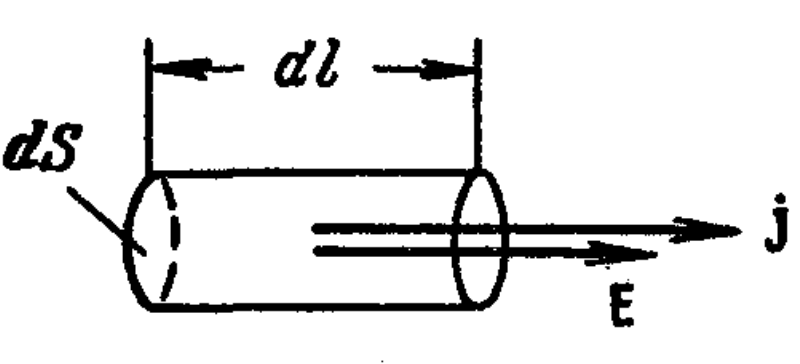
\includegraphics[scale=0.3]{e-01}
	\caption{Цилиндр}
	\label{e-01-cil}
\end{wrapfigure}
где $\sigma = 1/\rho$ - коэффициент электропроводности(проводимость материала).\\
\textbf{Границы применимости закона Ома}\\
При некоторых значениях напряженности электрического поля, созданного в газах, перемещающаяся заряженная частица может приобрести такую энергию, которой достаточно для того, чтобы вызвать вторичную ионизацию молекул. Число носителей зарядов при этом возрастает, удельная электропроводность изменяется. Вследствие этого пропорциональность между плотностью тока и напряженностью электрического поля нарушается. Отклонение от пропорциональности наблюдается и при искровом разряде в газах. Оба эти случая означают явное нарушение закона Ома.

Не подчиняется закону Ома и ток в электронных лампах, ток через контакт между двумя полупроводниками или полупроводником и металлом. Катастрофическим нарушением закона Ома является ток в сверхпроводниках.

Однако для металлов ни при каких условиях не удалось заметить отклонений от пропорциональности между плотностью тока и напряженностью электрического поля.
\end{document}